\chapter{Background}
\label{chap:background}
\glsreset{nn}
This chapter provides some background concepts to understand the material 
presented in this thesis. 
We start with a review about differential drive robots and their kinematics, 
providing some useful notions about the types of sensors used and finally 
summarising the theory of control (Section \ref{sec:ddr}).
We conclude with a refresh on \glspl{nn} (Section \ref{sec:nn}).

\section{Differential drive robots}
\label{sec:ddr}
\glsreset{icc}
The robot we use for this study is Thymio II, a non-holonomic differential drive 
robot.

A differential wheeled vehicle is mobile robot, that typically consists of a rigid 
body 
\begin{figure}[!htb]
	\centering
	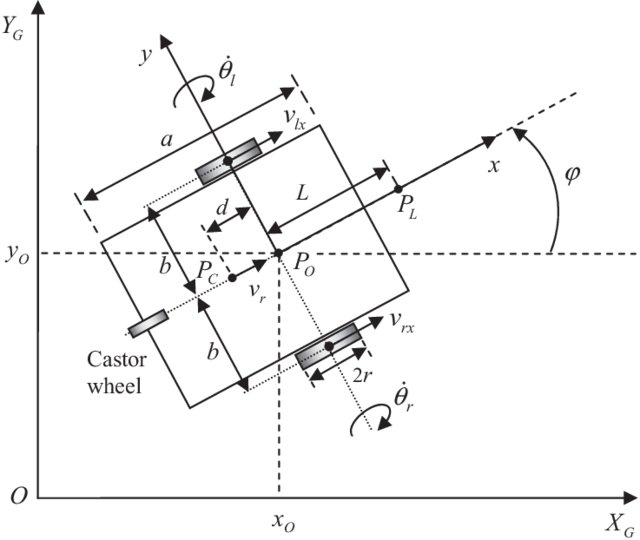
\includegraphics[width=.55\textwidth]{contents/images/Non-holonomic-differential-drive-mobile-robot}
	\caption[Non-holonomic differential drive mobile robot.]{Configuration of a 
		non-holonomic differential drive mobile robot 
		\cite[][]{shojaei2011adaptive}.}
	\label{fig:differentialdrive}
\end{figure}

\noindent
and a mobile base with a system of wheels that allows movement in the 
environment. 
Its movements are based on two, independently powered and 
controlled, fixed wheels, placed on either side of the robot body, with a common 
axis of rotation, and one passive caster wheel, whose job is to keep the robot 
statically balanced. 
Thus, both drive and steering functions are provided. In fact, it is possible to 
impose different values of velocity for the two fixed wheels, allowing the robot to 
rotate and move back and forth \cite[][]{siciliano2010robotics}. It is important to 
note that the robot is non-holonomic since it cannot translate laterally.

The \gls{icc}, is the point which lies along the horizontal axis, common to the left 
and right wheels, perpendicular to the plane of each wheel. Its position changes 
over time as a function of the individual wheel velocities, in particular of their 
relative difference. Since the rate of rotation $\omega$ is the same for both 
wheels, the following expressions hold:
\begin{Equation}[!h]
	\centering
	\begin{equation}
	\omega \, (R + b) = V_{rx}
	\end{equation}
	\begin{equation}
	\omega \, (R - b) = V_{lx}
	\end{equation}
	\caption[Right and left linear velocities of a differential drive robot.]{Right and 
	left linear velocities of a differential drive robot, computed as function of the 
	rotation rate, the distance between the wheels, and the distance from the 
	\gls{icc} and the robot reference point.}
	\label{eq:velocities}
\end{Equation}

\noindent
where $b$ is the distance between the centres of the two wheels, $V_{rx}$ and 
$V_{lx}$ are the right and left wheel velocities, and $R$ is the signed distance 
from the \gls{icc} to the midpoint between the wheels $P_O$ 
\cite[][]{dudek2010computational}. 
Moreover, at any specific time instant $t$ we can compute $R$ and  $\omega$ as 
follows:
\begin{Equation}[!h]
	\centering
	\begin{equation}
	R = b \, \frac{V_{rx} + V_{lx}}{V_{rx} - V_{lx}}
	\end{equation}
	\caption[Function to compute the distance from the ICC to the robot 
	reference point.]{Function to compute $R$, the signed distance from the 
	\gls{icc} to the midpoint between the wheels $P_O$, or robot reference point, 
	using the right and left linear velocities and the distance between the centres of 
	the two wheels.}
	\label{eq:r}
\end{Equation}

\begin{Equation}[!h]
	\centering
	\begin{equation}
	\omega = \frac{V_{rx} - V_{lx}}{2b}
	\end{equation}
	\caption[Function to compute the angular velocity of the robot.]{Function to 
	compute $\omega$, the angular velocity of the robot, using the right and left 
	linear velocities and the distance between the centres of the two wheels.}
	\label{eq:omega}
\end{Equation}

\bigskip
As a consequence, by varying the speed of the two wheels, $V_{rx}$ and 
$V_{lx}$, the trajectories that the robot takes changes as well:
\begin{itemize}
	\item $V_{rx} = V_{lx}$: if the same speed is set to both wheels, we have a 
	forward linear motion in a straight line. $R$ becomes infinite, and there
	is effectively no rotation $\omega = 0$.
	 
	\item $V_{rx} = - V_{lx}$: if both wheels are driven with equal speed but in the 
	opposite direction, we have a rotation about the midpoint of the wheel axis, or 
	in-place rotation. $R=0$, the \gls{icc} coincide with $P_O$ and $\omega = - 	
	\frac{V}{b}$.
	
	\item $V_{lx} = 0$: if the left wheel is not powered, we have a  
	counter-clockwise rotation about the left wheel. $R=b$ and 
	$\omega=\frac{V_{rx}}{2b}$.
	
	\item $V_{rx} = 0$: if the right wheel is not powered, we have a clockwise 
	rotation about the right wheel. $R=-b$ and $\omega=-\frac{V_{lx}}{2b}$.
\end{itemize}

Differential drive robots, however, are sensitive to slight changes in velocity, and 
even small errors can affect the robot trajectory. Moreover, they are also 
susceptible to variations in the ground.

\subsection{Sensors}
\label{subsec:sensors}

A significant feature of the Thymio II robot, is the a large number of sensors with 
which it is equipped.

The adoption of external sensing mechanism is of crucial importance to allow a 
robot to interact with its environment and achieve high-performance 
\cite[][]{fu1987robotics, siciliano2010robotics}. 

It is possible to classify the sensors in two principal categories, according to their 
function: \emph{proprioceptive} sensors, that measure the internal state and deal 
with the the detection of variables used for the control, such as the robot position, 
and \emph{exteroceptive} sensors that measure the external state of the 
environment, dealing with the detection of variables such as range and proximity, 
often used for robot guidance as well as object detection. 

For the purposes of this thesis we are interested in the study of proximity sensors, 
in particular the \gls{ir} sensors, that used by Thymio II.

Proximity sensors are an example of exteroceptive sensors: they gather 
information from the environment around the robot, such as distance to objects. 
They are 
also \emph{active} sensors: they emit their own energy, usually light, and measure 
the reflection. 
Among the advantages of this type of sensors is the fact that the infrared 
beams generated by the sources can be used unobtrusively, since they are 
invisible to the human eye.

\gls{ir} sensors are composed of an emitter, which radiates invisible infrared light, 
and a receiver, that measures the intensity of the reflection and the quantity of 
light that comes back.
If the reflection is strong enough — a large part of the light is reflected from 
the object and returns to the robot — it can be inferred that the obstacle is 
relatively close and lies within a certain range of the sensor, depending on 
the received intensity. If the object is farther away, only a small 
part of the light comes back \cite[][]{fu1987robotics}.
However, this estimate can be significantly affected by some property of the 
obstacle, such as its colour and reflectivity, but also by the presence of external 
light sources and the temperature of the environment — e.g. a black object 
reflects less light than a white one, placed at the same distance 
\cite[][]{mordechai2018elements}.

\subsection{Control theory}
\label{subsec:control}
The problem of controlling a robot is of a primary importance: to achieve a given 
task, an agent must acts based on the perception received from the environment. 
To do so, robots use a controller that takes decisions according to algorithms 
developed to accomplish the goal.

We can distinguish two main techniques of control: \emph{open-loop control} 
sets in advance the parameters of the algorithm and never observes the result of 
its actions to adjust them to the actual state, \emph{closed-loop control} or 
feedback-based control, measures the error between the desired state of the 
system and the actual one, and uses this feedback to to adjust the control and 
decide the next action to take \cite[][]{mordechai2018elements}.

These methods can be used to compute trajectories that lead the robot from an 
initial configuration to a final one. To achieve a more appropriate behaviour we 
are interested in the use of closed-loop control systems 
\cite[][]{siegwart2011introduction}.

\begin{figure}[!htb]
	\centering
	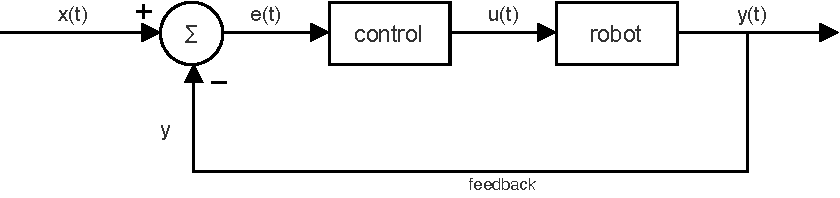
\includegraphics[width=.8\textwidth]{contents/images/closed-loop-control-system}
	\caption{Closed-loop control system.}
	\label{fig:closedloopcontrol}
\end{figure}
This model can be formally defined using the variables introduced below: 
\begin{itemize}
	\item $x(t)$, called command or set point (SP), represents the reference 
	value, or a desired output. It cannot be imposed directly on the robot, instead it 
	is transformed into a control value $u(t)$.
	
	\item $u(t)$, called control variable, is the output of the control and the 
	input of the robot.
	
	\item $y(t)$, called process variable (PV), represents an observable part of the 
	the actual state of the robot. It is the feedback signal combined with the set 
	point to compute the error value.

	\item $e(t)$ is the error. It is computed as the difference between the value of 
	the set point and the process variable, as shown in Equation 
	\ref{eq:systemerror}. The error is used to generate the new control signal $u(t)$.
	\begin{Equation}[!h]
		\centering
		\begin{equation}
		e(t) = x(t) - y(t)
		\end{equation}
		\caption{Calculation of the error value $e(t)$ of the system.}
		\label{eq:systemerror}
	\end{Equation}	
\end{itemize} 

The closed-loop control algorithms sometimes can be very sophisticated. For the 
purpose of this study, we design two algorithms, the first one is a \gls{pid} 
controller, while the second a Bang Bang controller.

The implementation of any feedback controller requires the availability of the 
robot configuration at each time instant. 

\subsubsection{Proportional (P) controller}
\label{subsubsec:pid}

Considering real situations in which agents do not have access to their states but 
only to their local observations, the controller we design for achieve the goal of 
the first task is a Proportional (P) Controller,  a particular variant of \gls{pid} 
Controller, with only the $K_p$ term, more details are provided in the Section 
\ref{subsubsec:manualtask1}.

The closed-loop control uses a feedback to adjust the control while the action 
takes place in proportion to the existing error. This function, given a desired 
output $x(t)$, or set point, produces an output $y(t)$, or process variable, such 
that the error $e(t)$ is obtained as the difference between the value of the set 
point and the process variable. Finally, the control variable $u(t)$ is the output of 
the \gls{pid} controller and is computed as follows:
\begin{Equation}[!h]
	\centering
	\begin{equation}
	u(t) = K_p * e(t)
	\end{equation}
	\caption[Proportioal PID controller.]{Proportional \gls{pid} controller.}
	\label{eq:pid}
\end{Equation}

The value of the proportional gain can be tuned to yield satisfactory 
performance so that the system is stable.

\subsubsection{Bang-bang controller}
\label{subsubsec:bangbang}
The controller we design to achieve the goal of the first task, of which more 
details are provided in the Section \ref{subsubsec:experttask1}, is a variant of the 
Bang-bang algorithm.

In this case we considered instead a situation in which agents have access to their 
states: given the set point and the variable measured, the goal and the actual 
position of the robot, the error is computed as the difference between the two 
quantities.
What we want to achieve is that the error is 0, to do so, when the error is negative, 
the robot should move forward to reach the goal, on the contrary if is positive it 
should move backwards. Its main feature is that the motor powers are turned to 
full forwards or full backwards depending on the sign of the error. 

This approach has many advantages, such as its simplicity and no need for 
calibration. 
However, since this controller is not always precise, especially when a derivative 
term is needed to avoid oscillations or when we are in steady-state, close to 
desired value, we implemented a variant that moves the the robot at full speed 
unless they are closer than a certain value, avoiding to approach the goal at full 
speed and overshoot it.

\section{Artificial Neural Networks}
\label{sec:nn}
In the field of \gls{ml}, \glspl{ann} are mathematical models based on the 
simplification of Biological Neural Networks \cite[][]{zou2008overview}. 

%FIXME missing reference of the image
\begin{figure}[htb]
	\centering
	\includegraphics[width=.7\textwidth]{contents/images/Neuron}
	\caption{Structure of a Biological Neuron.}
	\label{fig:bioneuron}
\end{figure}

A \gls{nn} can be considered as a dynamic system having the topology of an 
oriented graph, whose nodes model the neurons in a biological brain, while the 
edges represent the synapses — interconnections of information.
Each connection can transmit a signal from one artificial neuron to another,
which are typically aggregated in layers. The stimuli are received by a level of 
input nodes, called processing unit, which processes the signal and transmits it to 
other neurons connected to it.

As we anticipated, \glspl{nn} can be seen as mathematical models that define a 
function $f : X \rightarrow Y$. 
The network function of a neuron $f(x)$ is defined as a composition of
other functions $g_i(x)$, which can in turn be decomposed into others.
A widely used representation for the description of traditional \glspl{ann} is the 
weighted sum, shown in Equation \ref{eq:mathmodel}.

\begin{Equation}[!h]
	\centering
	\begin{equation}
	f(x)=\phi \bigg( \sum_{i}w_{i}x_i + \theta \bigg)
	\end{equation}
	\caption[Mathematical description of traditional \glspl{ann}.]{Function that 
	describes mathematically the traditional \glspl{ann} in terms of weighted sum.}
	\label{eq:mathmodel}
\end{Equation}
Each input signal $x_i$ is multiplied by its corresponding weight $w_{i}$, which 
assumes a positive or negative value depending on whether you want to excite or 
inhibit the neuron.
The bias $\theta$ varies according to the propensity of the neuron to activate, 
influencing its output.
Additionally, a predefined function $\phi$ can be applied, also called activation 
function, which is explained in the following paragraph.

\begin{figure}[htb]
	\centering
	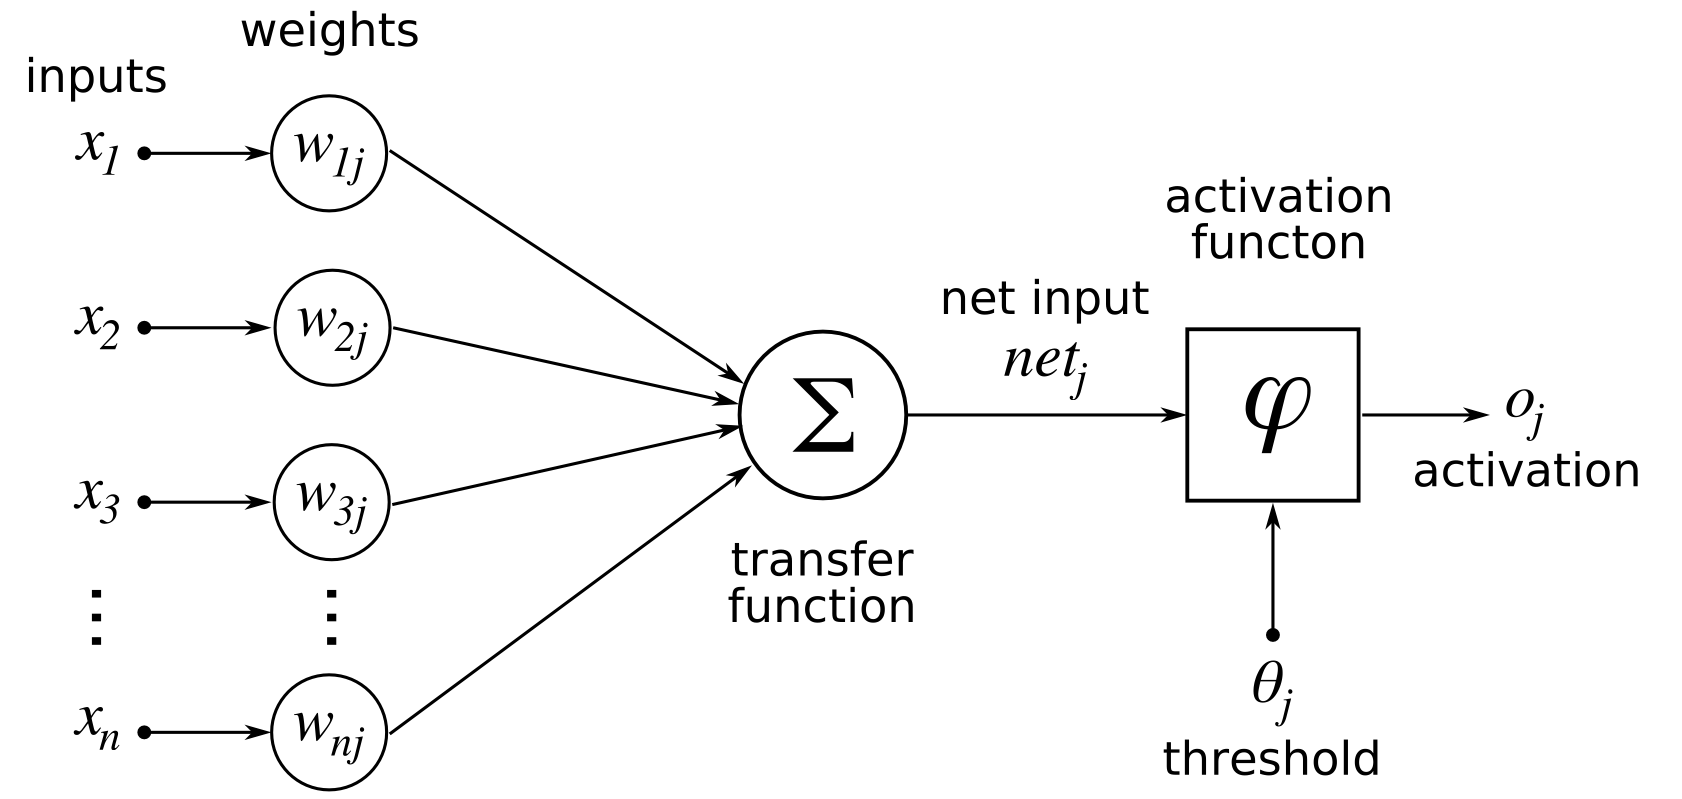
\includegraphics[width=.7\textwidth]{contents/images/ArtificialNeuronModel}
	\caption{Mathematical model of an Artificial Neuron.}
	\label{fig:neuron}
	\vspace{-0.5cm}
\end{figure}

\subsection{Activation functions}
\label{subsec:activationfun}

An activation function is a fundamental component of the model. It allows the 
network to learn non-linear transformations, in order to be able to compute 
non-trivial problems.
In the course of this study, we used two of the most popular activation functions  
in deep learning, the {hyperbolic tangent} (Tanh) \cite[][]{kalman1992tanh} 
and the {sigmoid} \cite[][]{han1995influence}, visualised in Figure 
\ref{fig:activation}.

\paragraph*{Tanh}
The tanh is a zero-centred function, whose range lies between $(-1, 1)$, and its 
output is given by the following formula:
\begin{Equation}[H]
	\centering
	\begin{equation}
	f(x)= \frac{\sinh (x)}{\cosh (x)} = \bigg( \frac{e^x - e^{-x}}{e^x + 
		e^{-x}}\bigg)
	\end{equation}
	\caption{Hyperbolic Tangent Function (Tanh).}
	\label{eq:tanh}
\end{Equation}

\paragraph*{Sigmoid}
The sigmoid models the frequency of the stimuli emitted by an inactive neuron, 
$\sigma(x)=0$, to one fully saturated with the maximum activation frequency, 
$\sigma(x)=1$. Its  output is given by the following formula:
\begin{Equation}[H]
	\centering
	\begin{equation}
	\sigma(x)= \frac{1}{1 + e^{-x}}
	\end{equation}
	\caption{Sigmoid Function.}
	\label{eq:sigmoid}
\end{Equation}

\begin{figure}[!htb]
	\begin{center}
		\begin{subfigure}[h]{0.495\textwidth}
			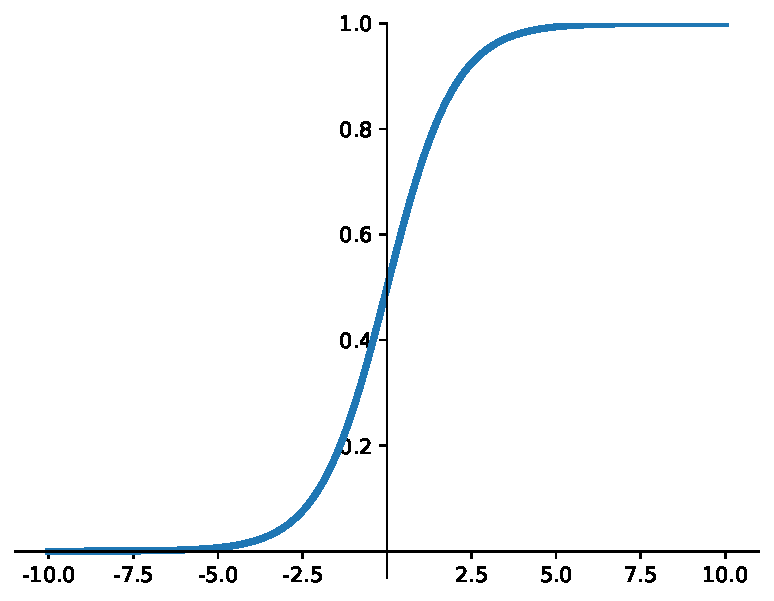
\includegraphics[width=.8\textwidth]{contents/images/sigmoid2}
			\caption{Tanh activation function.}
		\end{subfigure}
		\hfill
		\begin{subfigure}[h]{0.495\textwidth}
			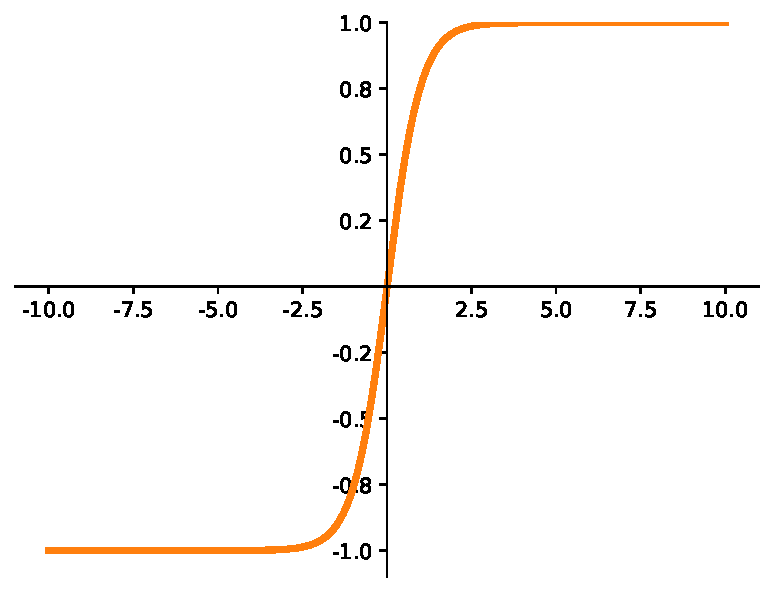
\includegraphics[width=.8\textwidth]{contents/images/tanh2}
			\caption{Sigmoid activation function.}
		\end{subfigure}
	\end{center}
	\caption{Trend of two non-linear activation functions.}
	\label{fig:activation}
\end{figure}

%\section{Architetture}
%\label{sec:architetture}
%
%I neuroni vengono organizzati in una struttura detta architettura della rete.
%I dati, partendo da un livello iniziale, chiamato layer di input, attraversano i 
%multipli strati interni della rete, gli hidden layer, raggiungendo l'ultimo livello 
%detto layer di output.
%
%Quando i collegamenti tra i neuroni formano una struttura senza cicli si parla di 
%reti \emph{feed-forward} \cite{svozil1997introduction}.
%
%\subsection{Layer fully-connected}
%\label{subsec:fc}
%
%Un’architettura molto comune nelle reti neurali è una struttura ``densa'', che 
%utilizza \emph{layer fully-connected}, in cui tutti i neuroni del livello precedente 
%sono collegati ad ogni neurone dello strato successivo 
%\cite{sainath2015convolutional}.
%
%Lo scopo di un layer completamente connesso è imparare combinazioni non 
%lineari di feature ad alto livello provenienti dal layer precedente. 
%Una struttura di questo tipo è però caratterizzata da un numero di connessioni 
%che cresce molto velocemente, causando un accrescimento del numero di 
%parametri che la rete deve apprendere.
%Questo comporta un aumento del costo computazionale e un alto rischio di 
%overfitting, approfondito nella sezione \ref{subsec:overfitting}.
%
%Per questo motivo questi vengono spesso sostituiti dai layer convoluzionali.

\subsection{Loss functions}
\label{subsec:lossfunctions}
\glsreset{mse}
\glsreset{bce}
The learning process is structured as a non-convex optimisation problem in which 
the aim is to minimise a cost function, which measures the distance between a 
particular solution and an optimal one.

In the course of this study we used two different objective functions, depending 
on the strategy to be adopted: to solve the first task, that can be modelled as a 
regression problem, we used the \gls{mse} \cite[][]{wang2009mean}, while for the 
second, that is a binary classification problem, we used the \gls{bce} 
\cite[][]{gomez2018understanding}.

\paragraph*{Mean Squared Error} 
The \gls{mse} computes the deviation between the values observed $\hat y_i$ and 
those predicted by the network $y_i$, over the number of predictions $n$, as 
shown in Equation \ref{eq:mse}.
\begin{Equation}[!htb]
	\centering
	\begin{equation}
	\mathtt{MSE} = \frac{\sum_{i=1}^n (y_i-\hat y_i)^2}{n}
	\end{equation}
	\caption{Mean Squared Error (MSE) loss function.}
	\label{eq:mse}
\end{Equation}
Formally, this criterion measures the average of squared error between 
predictions and targets, and learns to reduce it by penalising big errors in the 
model predictions.

\paragraph*{Binary Cross Entropy} 
The \gls{bce} is a combination of the sigmoid activation and the \gls{ce}. It sets up 
a binary classification problem between two classes, with the following 
formulation:

\begin{Equation}[!htb]
	\centering
	\begin{equation}
	\mathtt{BCE} = -\frac{1}{n} \sum_{i=1}^n y_i \cdot \log(\hat y_i) + (1-y_i) 
	\cdot \log(1 - \hat y_i)
	\end{equation}
	\caption[Binary Cross Entropy (BCE) loss function.\bigskip]{Binary Cross 
	Entropy 
	(\gls{bce}) loss function \cite[][]{sadowski2016notes}.}
	\label{eq:bce}
\end{Equation}

\noindent
where $\hat y_i$ is the $i$-th scalar value in the model output, $y_i$ is the 
corresponding target value, and $n$ is the number of scalar value in the model 
output\footnote{\url{https://peltarion.com/knowledge-center/documentation/modeling-view/build-an-ai-model/loss-functions/binary-crossentropy}}.
 
This loss function should return high values for bad predictions and low values for 
good ones.

\subsection{Optimisation algorithms}
\label{subsec:optimiser}
Optimisation algorithms are needed to minimise the result of a given objective 
function, which depends on the parameters the model has to learn during 
training.
They strongly influence the effectiveness of the learning process as they update 
and calculate the appropriate and optimal values of that model. 
In particular, the extent of the update is determined by the learning rate, which 
guarantees convergence to the global minimum, for convex error surfaces, and to 
a local minimum, for non-convex surfaces.

\paragraph*{Adam}

The optimiser we have chosen for this thesis project is Adam, {an algorithm for 
first-order gradient-based optimisation of stochastic objective functions, based 
on adaptive estimates of lower-order moments} \cite[][]{kingma2014adam, 
loshchilov2017decoupled}. 
